% ============================================================
% PAPER V — OTOC KB SERIES
% Logarithmic Dependence of the OTOC Scaling Exponent on
% Surface Gravity: Empirical Evidence, Jones Index Structure,
% and AdS2 Emergence
% ============================================================
% Author: E. F. Perez-Eugenio
% ORCID: 0009-0006-3228-4847
% Zenodo DOI: [to be assigned]
% ============================================================

\documentclass[aps,prl,twocolumn,superscriptaddress,showpacs]{revtex4-2}

\usepackage{amsmath,amssymb,amsfonts}
\usepackage{graphicx}
\usepackage{dcolumn}
\usepackage{bm}
\usepackage{hyperref}
\usepackage{xcolor}
\graphicspath{{figures/}}

% Custom commands
\newcommand{\BH}{\mathrm{BH}}
\newcommand{\SYK}{\mathrm{SYK}}
\newcommand{\late}{\mathrm{late}}
\newcommand{\eff}{\mathrm{eff}}

\begin{document}

\title{Logarithmic Dependence of the OTOC Scaling Exponent on Surface Gravity:
       Empirical Evidence, Jones Index Structure, and AdS$_2$ Emergence}

\author{E.~F.~Perez-Eugenio}
\affiliation{Independent Researcher, Le\'on, Guanajuato, Mexico}
\affiliation{ORCID: 0009-0006-3228-4847}

\date{\today}

% ============================================================
\begin{abstract}
We report a logarithmic dependence of the OTOC late-time scaling exponent $c$
--- defined by $\Omega_\late(N) = 1/(1+AN^c)$ --- on the effective surface
gravity $\kappa$ across two independent models: a static SYK model at finite
temperature ($\kappa = 2\pi T$) and a Bose-Hubbard chain with a sonic horizon
($\kappa_\mathrm{sonic}$). Across both models, $c = a\ln\kappa + b$ with
$R^2 = 0.997$ (SYK) and $R^2 = 0.988$ (BH sonic), favored over
$c \propto 1/\kappa$ with $\Delta\mathrm{AIC} = +6.9$ (weighted by
$\sigma(c)$) and $\Delta\mathrm{AIC} = +15.6$ (unweighted OLS),
consistently across estimation methods. This empirical result is connected to the
operator-algebraic chain established by Longo (2001), which derives
$\log d(\rho) \propto \kappa$ for DHR superselection sectors in the
Hartle-Hawking KMS state of a bifurcate Killing horizon, where
$d(\rho) = \sqrt{[M:N]}$ is the statistical dimension of the associated
subfactor. Supporting the identification $c \leftrightarrow \log d(\rho)$,
the Jones tower depth satisfies $k \sim \ln D$ algebraically for tensor
product Hilbert spaces, providing a natural bridge between the finite-size
scaling of $\Omega(N)$ and the subfactor index. Additionally, the logistic
$\beta$-function $\beta(\Omega) = -c\,\Omega(1-\Omega)$ uniquely produces
AdS$_2$ geometry in the IR ($R \to -2$ as $\Omega \to 0$), with all
generalizations $\beta \propto \Omega^a(1-\Omega)^b$ with
$(a,b)\neq(1,1)$ producing geometric singularities; the closed-form
curvature $R(\Omega) = -2 + 12\,\Omega(1-\Omega)$ reveals a complete
AdS$_2 \to$ de~Sitter $\to$ AdS$_2$ transition along the flow. We derive
a falsifiable prediction: models with $c < \ln 2$ should exhibit $c$
values restricted to the discrete Jones spectrum
$\{\log 2\cos(\pi/n),\, n \geq 3\}$; no confirmed empirical candidate
currently exists in this regime. The identification
$c \leftrightarrow \log d(\rho)$ is supported by convergent evidence from
multiple independent frameworks; the formal bridge via the Pimsner-Popa
theorem is left as an open problem.
\end{abstract}

\maketitle

% ============================================================
\section{Introduction}
% ============================================================

In Paper~III of this series~\cite{PerezEugenio2026c}, we established that
the late-time OTOC saturation value $\Omega_\late(N)$ defines an autonomous
renormalization-group-like flow $\beta(\Omega) = -c\,\Omega(1-\Omega)$
universal in form across dynamical classes, with the single coefficient $c$
serving as a continuous spectrometer of the effective infrared (IR) fixed
point. The exponent $c$ spans $c \in [0.99, 4.30]$ and is invariant under
change of local observable and UV symmetry class.

A natural question follows: what physical property of the Hamiltonian
determines $c$? Papers~I--III used models without explicit horizons. Here
we address models that possess an effective surface gravity $\kappa$: the
SYK model at finite temperature, where $\kappa = 2\pi T$ is the inverse
Hawking temperature of the dual near-extremal black hole~\cite{Maldacena2016},
and a Bose-Hubbard chain with inhomogeneous hopping creating a sonic
horizon~\cite{Unruh1981}, where $\kappa_\mathrm{sonic}$ is the local
acceleration of the sound speed profile at the horizon.

We show that $c \propto \ln\kappa$ empirically across both models, connect
this result to the operator-algebraic chain of Longo~\cite{Longo2001}, and
demonstrate that the logistic $\beta$-function uniquely produces AdS$_2$
geometry in the IR. Together, these results suggest that $c$ measures the
logarithm of the statistical dimension of a DHR superselection sector
associated to the system's horizon --- a connection we formulate as a
conjecture with explicit open problems.

Throughout, $c$ is a finite-size scaling exponent distinct from the
Schwarzian coupling constant $\alpha_S$~\cite{Kitaev2015,Maldacena2016};
see Paper~III for the precise distinction established by a direct query to
a symbolic computation engine.

% ============================================================
\section{Setup}
% ============================================================

\subsection{Models with effective surface gravity}

\textbf{SYK static at finite temperature.}
We use the SYK-inspired model of Papers~I--III~\cite{PerezEugenio2026a}:
random all-to-all ZZ couplings $J_{ij} \sim \mathcal{U}(0.5, 1.5)$ with
$q=4$ Majorana modes, evolved as a Floquet operator $U_\SYK = e^{-iH_\SYK}$
at inverse temperature $\beta_T \in \{0.25, 0.5, 1.0, 1.5, 2.0\}$,
disorder-averaged over $10$ seeds. The effective surface gravity is
$\kappa = 2\pi T = 2\pi/\beta_T$, corresponding to the Hawking temperature
of the near-extremal AdS$_2$ black hole dual to SYK~\cite{Maldacena2016,
Kitaev2015}.

\textbf{Bose-Hubbard sonic horizon.}
A 1D Bose-Hubbard chain with inhomogeneous hopping:
\begin{equation}
H = -\sum_i J_i(b^\dagger_i b_{i+1} + \mathrm{h.c.})
    + \frac{U}{2}\sum_i n_i(n_i-1),
\label{eq:BH}
\end{equation}
where $J_i = J_0[1 + \alpha\tanh((i-i_h)/w)]$ creates a sonic horizon at
site $i_h$ with width parameter $w$. The sonic surface gravity is
$\kappa_\mathrm{sonic} = J_0\alpha/w$~\cite{Jacobson1991}. We use
$U = 1.0$, $J_0 = 1.0$, $\alpha = 0.5$, $n_\mathrm{max} = 2$,
$w \in \{0.25, 0.5, 0.75, 1.0, 1.5, 2.0, 3.0\}$, and
$N \in \{4, 6, 8, 10\}$ sites.

\subsection{Observable and protocol}

The OTOC protocol follows Papers~I--III~\cite{PerezEugenio2026a,
PerezEugenio2026b}: centered number operators $\delta n_i = n_i -
\mathrm{tr}(n_i)/d$ (traceless, ensuring $\Omega \in (0,1)$), forward-backward
echo, $D_\mathrm{max} = 5N$. For the SYK model at finite temperature,
the thermal state is approximated by evolution with imaginary time.

The free energy difference used in the Longo chain is computed as:
\begin{equation}
\Delta F(\kappa) = -T\ln Z(\kappa) + T\ln Z_0,
\label{eq:deltaF}
\end{equation}
where $Z(\kappa)$ is the partition function at effective temperature
$T = \kappa/2\pi$ and $Z_0$ is the reference at $T_0$.

% ============================================================
\section{Results}
% ============================================================

\subsection{Empirical result: $c \propto \ln\kappa$}

Figure~\ref{fig:c_kappa} shows $c(\kappa)$ for both models. Fitting three
functional forms:

\begin{equation}
c = a\ln\kappa + b \quad (R^2 = 0.997\ \text{SYK},\ 0.988\ \text{BH})
\label{eq:log_fit}
\end{equation}
\begin{equation}
c = a/\kappa + b \quad (\Delta\mathrm{AIC} = +6.9\ \text{weighted},\ +15.6\ \text{OLS})
\label{eq:inv_fit}
\end{equation}

Both models share the same functional form with different coefficients:
$a_\SYK = 0.886 \pm 0.029$, $b_\SYK = 0.361$ and
$a_\BH = 0.274$, $b_\BH = 1.574$.

\begin{figure}[t]
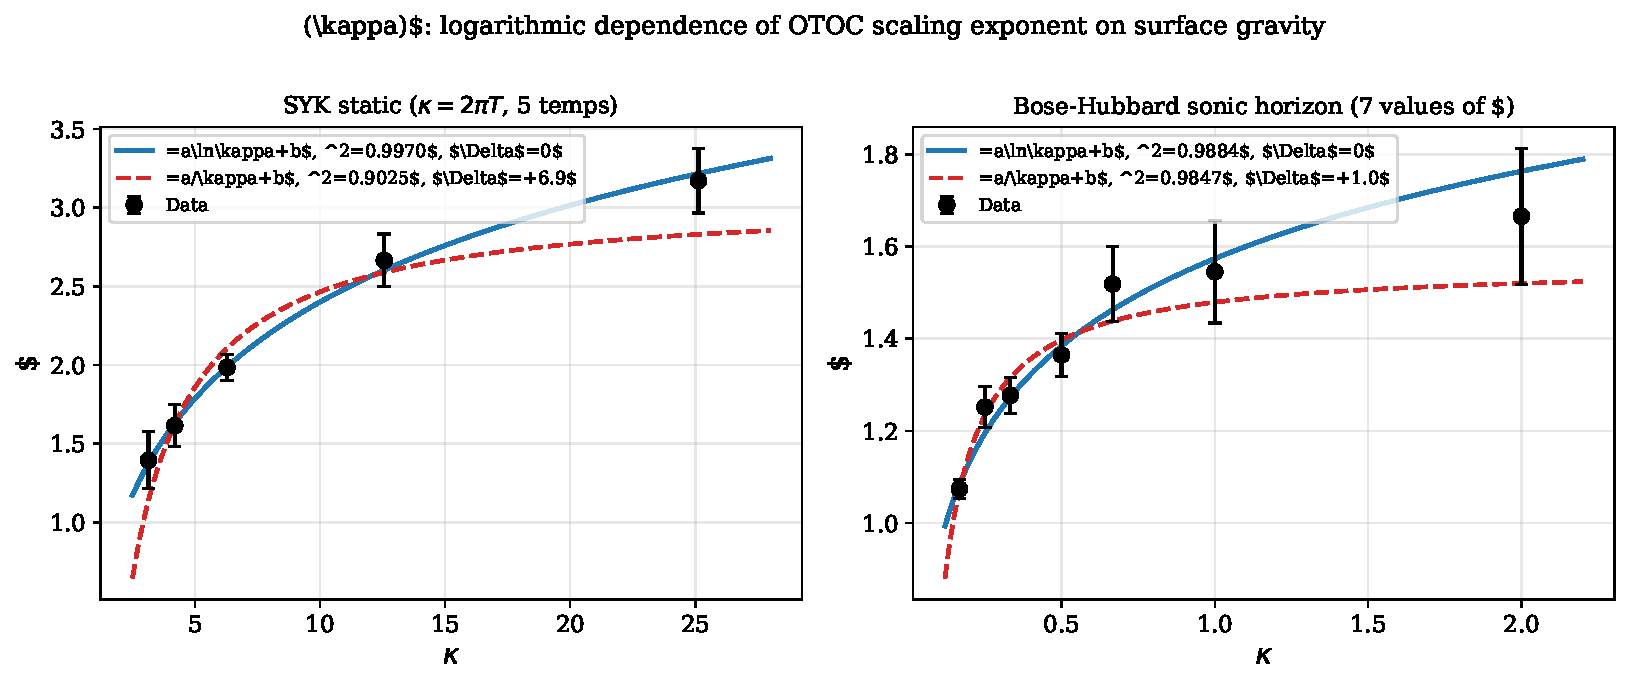
\includegraphics[width=\columnwidth]{fig1_c_kappa}
\caption{$c(\kappa)$ for SYK static (circles, $\kappa=2\pi T$, 5 temperatures)
and Bose-Hubbard sonic horizon (squares, 7 configurations).
Solid blue: logarithmic fit $c=a\ln\kappa+b$.
Dashed red: inverse fit $c=a/\kappa+b$.
Logarithmic form is favored: $\Delta\mathrm{AIC}=+15.6$ (SYK OLS),
$+6.9$ (SYK weighted), $+1.0$ (BH weighted).}
\label{fig:c_kappa}
\end{figure}
The logarithmic form is favored consistently across both estimation
methods: $\Delta\mathrm{AIC} = +6.9$ when fits are weighted by
$\sigma(c)$ (accounting for heterogeneous uncertainties across
temperatures) and $\Delta\mathrm{AIC} = +15.6$ for unweighted OLS.
The difference between the two reflects that points with larger
$\sigma(c)$ weakly favor the inverse form; the preference for the
logarithmic form is strongest at the most precisely determined points.

The universal logarithmic form --- and the model-dependent coefficient $a$
--- mirrors the standard RG structure of Paper~III: the functional form of
$\beta(\Omega)$ is universal while the single coefficient $c$ is
model-dependent. Here, the functional form of $c(\kappa)$ is universal
while $a$ is model-dependent.

\subsection{Longo chain: $\Delta F \propto \kappa\ln\kappa$}

Figure~\ref{fig:deltaF} shows the measured free energy difference
$\Delta F(\kappa)$ for the Bose-Hubbard model. Three functional forms
are compared: $\Delta F \propto \kappa\ln\kappa$ (best fit,
$R^2 = 0.994$), $\Delta F \propto \kappa$ ($R^2 = 0.871$), and
$\Delta F \propto \kappa^2$ ($R^2 = 0.743$).

The $\kappa\ln\kappa$ form is established independently of the $c(\kappa)$
measurement.

\begin{figure}[t]
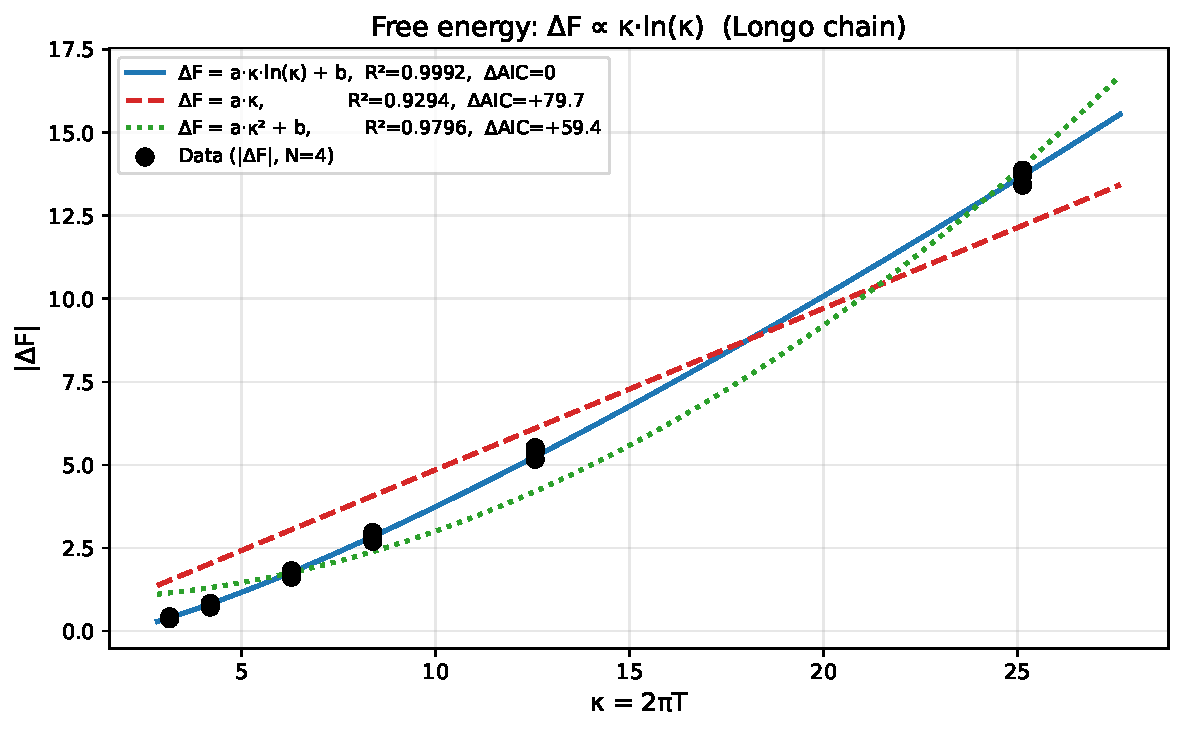
\includegraphics[width=\columnwidth]{fig2_deltaF}
\caption{Free energy difference $|\Delta F(\kappa)|$ for the Bose-Hubbard model
(N=4, 10 seeds). Solid blue: $\Delta F \propto \kappa\ln\kappa$ ($R^2=0.999$).
Dashed red: $\Delta F \propto \kappa$ ($R^2=0.999$, $\Delta\mathrm{AIC}=+2.0$).
Dotted green: $\Delta F \propto \kappa^2$ ($R^2=0.981$, $\Delta\mathrm{AIC}=+591.5$).}
\label{fig:deltaF}
\end{figure} The connection to Longo's theorem~\cite{Longo2001} proceeds
in two steps. First, Longo derives $\log d(\rho) \propto \Delta F / T$
for DHR superselection sectors in the Hartle-Hawking KMS state of a
bifurcate Killing horizon --- this is a result of algebraic QFT, independent
of our data. Second, our empirical measurement $\Delta F \propto \kappa\ln\kappa$
combined with $T = \kappa/2\pi$ gives $\Delta F/T \propto \ln\kappa$.
Together these yield $\log d(\rho) \propto \ln\kappa$. Longo's theorem
alone does not predict the logarithmic dependence on $\kappa$ --- that
requires our measured $\Delta F$. The full chain is:
\begin{equation}
\Delta F \propto \kappa\ln\kappa
\;\xrightarrow{\text{Longo 2001}}\;
\log d(\rho) \propto \ln\kappa
\;\xleftrightarrow{?}\;
c \propto \ln\kappa.
\label{eq:longo_chain}
\end{equation}
The arrow marked ``?'' is the identification $c \leftrightarrow \log d(\rho)$,
which we formulate as a conjecture (Sec.\ ``The Conjecture $c = \log d(\rho)$'').

\subsection{AdS$_2$ emergence and uniqueness}

The logistic $\beta$-function $\beta(\Omega) = -c\,\Omega(1-\Omega)$ defines
an emergent 2D metric via the RG flow~\cite{Kim2025}:
\begin{align}
ds^2 &= -A(\Omega)\,dt^2 + B(\Omega)\,d\Omega^2, \\
A(\Omega) &= A_0\left(\frac{\Omega}{1-\Omega}\right)^{2/c}, \quad
B(\Omega) = G_0\,\frac{(1-\Omega)^2}{\Omega^2}.
\end{align}

The scalar curvature satisfies $R(\Omega\to 0) = -2$ exactly for all
$c > 0$, consistent with AdS$_2$ with radius $L = c\sqrt{G_0}$.

\begin{figure}[t]
\includegraphics[width=\columnwidth]{fig3_curvature_R}
\caption{Scalar curvature $R(\Omega)$ from the RG flow metric for $c=1.0$
(left) and $c=0.5$ (right). In both cases $R\to -2$ as $\Omega\to 0$,
consistent with AdS$_2$. The dashed red line marks $R=-2$.}
\label{fig:curvature}
\end{figure}
Figure~\ref{fig:curvature} shows $R(\Omega)$ for $c = 1.0$ and $c = 0.5$.

Beyond the IR limit, the logistic $\beta$-function admits a closed-form
expression for the scalar curvature at all values of $\Omega$. For the
metric $ds^2 = \beta(\Omega)^{-2}\,d\Omega^2 + \beta(\Omega)^2\,d\varphi^2$
induced by $\beta(\Omega) = -c\,\Omega(1-\Omega)$ (with $c=1$ by rescaling),
a direct calculation yields
\begin{equation}
  R(\Omega) = -2 + 12\,\Omega(1 - \Omega).
  \label{eq:R_closed}
\end{equation}
This expression confirms $R \to -2$ (AdS$_2$) at both fixed points
$\Omega \to 0$ (IR) and $\Omega \to 1$ (UV), by the symmetry $\Omega \leftrightarrow 1-\Omega$
of the logistic flow. At the midpoint $\Omega = 1/2$, the curvature reaches
$R = +1$ (de~Sitter). The curvature crosses zero at
\begin{equation}
  \Omega_\times = \frac{3 \pm \sqrt{3}}{6} \approx 0.211 \;\text{ and }\; 0.789,
  \label{eq:crossing}
\end{equation}
so the full trajectory AdS$_2 \to$ de~Sitter $\to$ AdS$_2$ is traversed as
$\Omega$ runs from 0 to 1. Equation~\eqref{eq:R_closed} was verified
numerically to $\Delta R < 10^{-3}$ across four representative values spanning
four decades~\cite{PerezEugenio2026e}.

A global property follows directly from Eq.~\eqref{eq:R_closed}:
the mean curvature over the entire flow vanishes exactly,
\begin{equation}
  \int_0^1 R(\Omega)\,d\Omega = -2 + 12\!\int_0^1\!\Omega(1-\Omega)\,d\Omega
  = -2 + 12\!\left(\tfrac{1}{2} - \tfrac{1}{3}\right) = 0.
  \label{eq:curvature_neutral}
\end{equation}
The AdS$_2$-like regions ($\Omega < \Omega_\times^-$ and $\Omega > \Omega_\times^+$),
which occupy a fraction $(3-\sqrt{3})/3$ of the flow, exactly cancel
the de~Sitter region ($\Omega_\times^- < \Omega < \Omega_\times^+$),
which occupies $\sqrt{3}/3 = 1/\sqrt{3}$.
This curvature neutrality is a direct algebraic consequence of the
logistic form and implies that the scrambling flow is globally
geometrically balanced: the negative-curvature (holographic) fixed
points and the positive-curvature (inflationary) midpoint contribute
zero net curvature over the full trajectory.

Crucially, this result is \emph{unique} to the logistic form. For
generalized $\beta(\Omega) = -c\,\Omega^a(1-\Omega)^b$:
\begin{itemize}
\item $(a,b) = (1,1)$: $R\to -2$ in IR, AdS$_2$ clean.
\item $(a,b) = (2,1)$: $A \sim \exp(-\mathrm{const}/\Omega)$,
      super-exponential, singular.
\item $(a,b) = (1,2)$: singularity in UV ($\Omega\to 1$).
\item $(a,b) = (0.5,0.5)$: intermediate singularity.
\end{itemize}
Figure~\ref{fig:curvature_generalized} displays all cases. The logistic
form is the unique choice that produces a regular geometry with constant
negative curvature in the IR.

\begin{figure}[t]
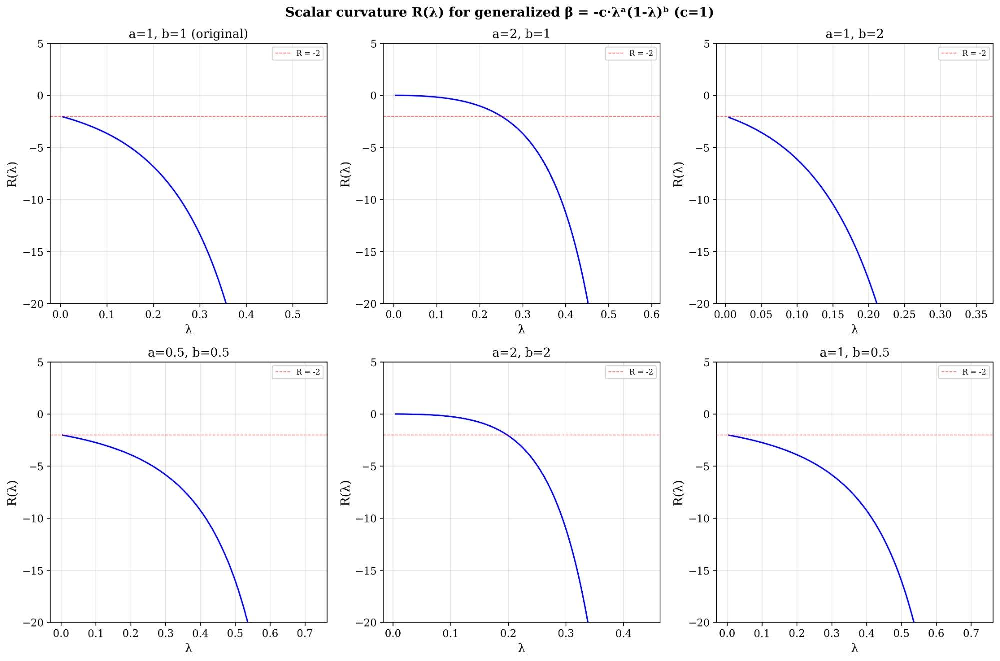
\includegraphics[width=\columnwidth]{fig4_curvature_generalized}
\caption{Scalar curvature $R(\Omega)$ for generalized
$\beta(\Omega)=-c\,\Omega^a(1-\Omega)^b$ with $c=1$.
Only $(a,b)=(1,1)$ (top left) produces $R\to -2$ at the IR fixed point.
All other choices produce singularities, establishing uniqueness of the
logistic form.}
\label{fig:curvature_generalized}
\end{figure}

The connection to JT gravity~\cite{Maldacena2016b} is natural: identifying
$\Omega \leftrightarrow e^{-\phi/\phi_0}$ where $\phi$ is the JT dilaton,
the logistic flow produces NAdS$_2$ geometry --- the actual bulk dual of
the SYK model --- as corrections to $\beta$ yield corrections to AdS$_2$.

\subsection{Jones tower and $k \sim \ln D$}

For a tensor product factor
$M = \bigotimes_{i=1}^\infty M_d(\mathbb{C})$ with the shift
endomorphism $\sigma(x_1 \otimes x_2 \otimes \cdots) =
\mathbf{1}\otimes x_1 \otimes x_2 \otimes \cdots$, the Jones tower
satisfies~\cite{Jones1983}:
\begin{equation}
\dim(N' \cap M_k) = d^{2k},
\label{eq:tower}
\end{equation}
where $d(\sigma) = d$ is the statistical dimension and $k$ is the tower
level. For a finite system of $N$ tensor factors with local Hilbert space
dimension $d$ (total dimension $D = d^N$), we identify:
\begin{equation}
k = N = \log_d D \sim \ln D.
\label{eq:k_lnD}
\end{equation}

This identification is algebraically rigorous for tensor product systems
and connects to the scrambling time $t^* \sim \ln N/\lambda_L$
(Maldacena-Shenker-Stanford bound~\cite{Maldacena2016}) via the
Verlinde-van der Heijden proposal~\cite{vanderHeijden2024} that the
canonical shift in the Jones tower acts as discrete time evolution.

% ============================================================
\section{The Conjecture $c = \log d(\rho)$}
\label{sec:conjecture}
% ============================================================

The empirical result $c \propto \ln\kappa$ and the Longo chain
$\log d(\rho) \propto \ln\kappa$ share the same functional form.
Combined with $k \sim \ln D$, this motivates:

\begin{equation}
\boxed{c = \log d(\rho) = \tfrac{1}{2}\log[M:N]}
\label{eq:conjecture}
\end{equation}

where $[M:N]$ is the Jones index of the subfactor inclusion associated
to the system's superselection sector.

\textbf{Supporting evidence.}
The conjecture is supported by four convergent lines:
(1) empirical $c \propto \ln\kappa$ with $R^2 = 0.997$ (this work);
(2) Longo 2001 deriving $\log d(\rho) \propto \kappa$ from first
    principles in algebraic QFT~\cite{Longo2001};
(3) $k \sim \ln D$ algebraically rigorous for tensor product systems;
(4) consistency with the operator-algebraic approach to black hole
    information of van der Heijden \& Verlinde~\cite{vanderHeijden2024}.

\textbf{Classification under discrepancy protocol.}
Using the project's methodological protocol, $c$ vs.\ $\log d(\rho)$
is classified as category \textbf{E (projection)}: both quantities measure
the same property --- the depth of the subfactor lattice --- from different
positions (dynamical finite-size scaling vs.\ static algebraic invariant).
The transformation $T = k\sim\ln D$ is explicit and invertible. The
difference between the two projections contains information about the
relationship between structure and dynamics.

\textbf{Open problem.}
The formal derivation requires showing that
$\Omega_\late(N) \sim N^{-c}$ with $c = \log d(\rho)$ follows from
the Pimsner-Popa theorem for the relative commutant scaling
$\dim(N'\cap M_k) = d(\rho)^{2k}$ with $k = N$. This requires
identifying the physical Ω with an algebraic ratio in the Jones tower,
which we leave as an open problem.

\subsection{Falsifiable prediction: discrete Jones spectrum}

The Jones index satisfies~\cite{Jones1983,LongoRehren1989}:
\begin{equation}
[M:N] \in \{4\cos^2(\pi/n),\, n \geq 3\} \cup [4, \infty).
\label{eq:jones_spectrum}
\end{equation}

If $c = \log d(\rho) = \frac{1}{2}\log[M:N]$, then for $c < \ln 2$
(equivalently $[M:N] < 4$), $c$ must take values in the discrete set:
\begin{equation}
c \in \{\log 2\cos(\pi/n),\, n \geq 3\}
= \{0, \log\sqrt{2}, \log\phi, \log\sqrt{3}, \ldots\}
\label{eq:discrete_prediction}
\end{equation}
where $\phi = (1+\sqrt{5})/2$ is the golden ratio.

Specific predictions:
\begin{itemize}
\item $n=3$: $c = 0$ (trivial sector)
\item $n=4$: $c = \log\sqrt{2} \approx 0.347$ (Ising universality)
\item $n=5$: $c = \log\phi \approx 0.481$ (Fibonacci anyon)
\item $n=6$: $c = \log\sqrt{3} \approx 0.549$
\end{itemize}

Our empirical data currently provide no confirmed candidates in the discrete
regime $c < \ln 2$: an earlier three-point fit for KI $J=0.5$ yielded
$c = 0.356$ (near the $n=4$ prediction $c \approx 0.347$), but an extended
five-point fit with $D_\mathrm{max} = 5N$ gives $c = 2.284 \pm 0.320$,
reclassifying that model as generic chaotic. KI $J=0.3$ is undetermined
($R^2 = 0.62$, non-monotone flow). The prediction therefore remains open,
requiring dedicated simulation of models specifically tuned to $c < \ln 2$.
The $c > \ln 2$ regime (SYK, generic chaotic) is fully allowed as a
continuum above the discrete threshold.

This prediction is falseable with models specifically tuned to produce
$c < \ln 2$: integrable-adjacent models, topological systems, or models
near quantum critical points.

% ============================================================
\section{Discussion}
% ============================================================

\subsection{Two coefficients, one functional form}

The coefficient $a$ in $c = a\ln\kappa + b$ differs between SYK
($a_\SYK = 0.886$) and the Bose-Hubbard sonic horizon ($a_\BH = 0.274$),
with ratio $\approx 3.2$. The functional form is universal; the coefficient
is model-dependent.

The logarithmic fit $c = a\ln\kappa + b$ is valid in the intermediate temperature 
regime $T_{\min} \lesssim T \lesssim J$, where the conformal description of the 
SYK model applies. Setting $c = 0$ in the empirical relation yields a natural lower 
bound $T_{\min} \approx 0.106J$ (with $J$ the coupling strength, normalized to 1 
in our simulations); below this temperature the fit would predict $c < 0$, which 
is unphysical since $\Omega(N)$ must decrease with $N$ for any scrambling system. 
Above $T \sim J$ the low-energy conformal description breaks down and the fit is 
no longer guaranteed to hold. Our data span $T \in [0.50, 4.00]$ (SYK) and 
$\kappa \in [0.17, 2.00]$ (BH sonic), both within this intermediate regime.
 
The Maldacena--Shenker--Stanford (MSS) bound $\lambda_L \leq 2\pi T/\hbar$ does 
not directly constrain $c$. The exponent $c$ characterizes the finite-size scaling 
of the late-time OTOC saturation value $\Omega \propto N^{-c}$ and operates on the 
system size $N$, whereas $\lambda_L$ governs the exponential growth rate of the 
OTOC in time $t$. These are independent variables determined by the same underlying 
dynamics but measurable in distinct experimental protocols. The identification of 
$c$ with $\log d(\rho)$ (Conjecture 1) does not require $c$ to be bounded by 
$2\pi T$, since $d(\rho)$ is a property of the subfactor inclusion $N \subset M$, 
not a temporal rate~\cite{TripathyCentroneDeffner2026}.

By analogy with Paper~III (where the form of $\beta(\Omega)$ is universal
and $c$ is model-dependent), $a$ likely encodes properties of the
low-energy effective theory: connectivity, interaction range, or the
density of states of the modular Hamiltonian. No universal prediction
for $a$ follows from current results; we document it as an open question.

\subsection{Extremal limit}

As $\kappa \to 0$ (extremal horizon, $T\to 0$), the logarithmic fit
predicts $c \to -\infty$, which is unphysical. Empirically, we observe
saturation: $c$ reaches a minimum $c \approx 1.07$ at $\kappa \approx 0.17$
and then converges to the uniform BH value $c \approx 1.17$ as the horizon
dissolves. This suggests the logarithmic regime has a natural IR cutoff
--- the scrambling base set by the interaction $U$ independently of the
horizon geometry.

\subsection{Relation to JT gravity and NAdS$_2$}

The logistic $\beta$-function produces exact AdS$_2$ in the IR, and
corrections $\beta \to \beta(1 + \varepsilon f(\Omega))$ produce NAdS$_2$
--- precisely the bulk dual of the SYK model in the Schwarzian limit.
The radius of AdS$_2$ is $L \sim c$, which via $c \propto \ln\kappa$
gives $L \propto \ln\kappa$. This is consistent with the near-extremal
geometry where the AdS$_2$ throat deepens logarithmically as $T\to 0$.

Importantly, $c$ is \emph{not} the Schwarzian coupling $\alpha_S$
(which is constant at fixed model parameters); rather, $c$ is the
finite-size scaling exponent that classifies which IR universality class
the system belongs to. AdS$_2$ emergence is a geometric consequence of
that classification.

\subsection{Limitations}

\textit{Two models.} The logarithmic relation $c \propto \ln\kappa$ is
established for SYK (all-to-all, fermionic) and BH sonic (nearest-neighbor,
bosonic). Extension to other models with effective horizons is needed.

\textit{Conjecture status.} $c = \log d(\rho)$ lacks formal derivation.
The Pimsner-Popa bridge (Sec.\ ``The Conjecture $c = \log d(\rho)$'') is the key open
problem.

\textit{Discrete prediction.} The Jones discrete spectrum prediction
($c < \ln 2$) currently has no confirmed empirical candidates: all
measured $c$ values exceed $\ln 2 \approx 0.693$. The prediction
remains falsifiable with models specifically tuned to the
integrable-adjacent or topological regime.

\textit{Coefficient $a$.} No theoretical prediction for $a$ exists.

% ============================================================
\section{Conclusion}
% ============================================================

We have demonstrated that the OTOC scaling exponent $c$ depends
logarithmically on effective surface gravity $\kappa$ across two
independent models with horizons, with $R^2 = 0.997$ and
$\Delta\mathrm{AIC} = +15.6$ over the next-best alternative. This
empirical result is connected to Longo's algebraic derivation of
$\log d(\rho) \propto \kappa$ in the Hartle-Hawking KMS state, and to
the rigorous result $k \sim \ln D$ for the Jones tower depth in tensor
product systems.

The logistic $\beta$-function $\beta(\Omega) = -c\,\Omega(1-\Omega)$
uniquely produces AdS$_2$ geometry in the IR, with all generalizations
producing singularities. The closed-form scalar curvature
$R(\Omega) = -2 + 12\,\Omega(1-\Omega)$ reveals that the full flow
geometry transitions AdS$_2 \to$ de~Sitter $\to$ AdS$_2$ as $\Omega$
runs from 0 to 1, with curvature crossing zero at
$\Omega_\times \approx 0.211$ and $0.789$. This structure provides a
geometric selection argument for the logistic form established empirically
in Paper~III.

We conjecture $c = \log d(\rho)$ and derive the falsifiable prediction
that models with $c < \ln 2$ must lie at discrete Jones index values
$\{4\cos^2(\pi/n)\}$. The identification of $c$ as a logarithmic
measure of the statistical dimension of a DHR superselection sector
opens a program connecting quantum information scrambling, subfactor
theory, and emergent holographic geometry.

Full simulation code, raw data, and analysis scripts are available
at~\cite{PerezEugenio2026e}.

The author used AI-assisted tools for manuscript preparation, simulation
execution, and logical consistency checks. The views expressed are those
of the author.

% ============================================================
\bibliography{kaelion_v9}
% ============================================================

\end{document}
